\section{Splines}

\mode<article>

Este problema ya ha sido tratado en el apunte ``Cuentas 
de Interpolación''. Aquí usaremos los resultados que habíamos obtenido allí.
simplemente recordaremos que tenemos una serie de puntos experimentales 
por lo que queremos hacer pasar una función definida a tramos. 

\mode*
\begin{frame}<presentation>[label=FrameDefinicionSplines]
  \frametitle{Splines}
  \begin{equation}
    \begin{split}
    { (X_i, Y_i) }_{i = 1 \dots N}\\
      I_i = \left[ X_i , X_{i+1} \right] \\
      f_i = a_i (x - X_i)^3 + b_i (x-X_i)^2 + c_i (x-X_i) + d_i
    \end{split}
  \end{equation}
\end{frame}

\mode<article>
En cada intervalo $I_i$ vale el polinomio $f_i$ de grado 3. A estos polinomios
se les pide que sean continuos y que la primer y segunda derivada. Eso 
desemboca en un sistema de ecuaciones que termina en un sistema lineal para
los coeficientes $b_i$ . 

\mode*
\begin{frame}[label=FrameSistemaEcuacionesSplines]
  \frametitle<presentation>{Sistema De Ecuaciones para Splines}

  %  \includegraphics[width=\textwidth,page=4]{Resumen/GUIA1-Resumen-2018.pdf}
  \tiny
  \begin{equation}
   \begin{split}
      \begin{pmatrix}
	1 &     0      &    0    & 0 & \dots & 0 & 0 & 0 & 0 \\
	h_1& 2(h_2+h_1)& h_2     & 0 & \dots & 0 & 0 & 0 & 0 \\
	0  &  h_2  & 2(h_3+h_2) &h_3 & \dots & 0 & 0 & 0 & 0 \\
	\hdotsfor{9}\\
	0 & 0 & 0 & 0 & \cdots & h_{N-3} & 2(h_{N-2}+h_{N-3}) & h_{N-2} & 0 \\
	0 & 0 & 0 & 0 & \cdots & 0 & h_{N-2} &2(h_{N-1}+h_{N-2}) & h_{N-1} \\
	0 &     0      &    0    & 0 & \dots & 0 & 0 & 0 & 1
      \end{pmatrix} 
       \\
      \times 
      \begin{pmatrix}
	b_1 \\ b_2 \\ b_3 \\ \vdots \\ b_{N-2} \\ b_{N-1} \\ b_{N}
      \end{pmatrix} 
      = 
      3
      \begin{pmatrix}
	0 \\ 
	\dfrac{ Y_3 - Y_2 }{h_2} - \frac{ Y_2 - Y_1 }{h_1} \\
	\vdots \\
	\dfrac{ Y_N - Y_{N-1} }{h_{N-1}} - \frac{ Y_{N-1} - Y_{N-2} }{h_{N-2}} \\
	0
      \end{pmatrix}
    \end{split}
  \end{equation}
\end{frame}

\mode<article> 

Luego, al resolver el sistema de ecuaciones que sale de las condiciones
de borde para cada $f_i$ , tenemos las soluciones para $a_i$ y $c_i$ a partir de los 
$b_i$

\mode*

\begin{frame}[label=FrameEquationRecurrencias]
  \frametitle<presentation>{Coeficientes $a_i$ y $c_i$}
  \begin{equation}
    \begin{aligned}
      d_i =& Y_i \\
      a_i =& \frac{1}{3} \dfrac{ b_{i+1} - b_i }{h_i} \\
      c_i =& \dfrac{ Y_i - Y_{i-1} }{ h_{i-1} } - b_{i-1} h_{i-1}  - a_{i-1} h_{i-1} ^2
    \end{aligned}
  \end{equation}


\end{frame}
\mode<article>

Con estos datos podemos completar la escritura de los $N-1$ polinomios
necesarios. De esta manera, podemos graficar en cada intervalo 
el tramo correspondiente de la función como se muestra en la
\autoref{FiguraSplinesArmadas}. Debe notarse que cada polinomio vale solo
en su intervalo de definición, como se observa en la \autoref{FiguraSplinesExtendidos}.
Fuera de su propio intervalo, cada polinomio constituye una aproximación pobre
a los datos originales. 

\mode*
\begin{frame}[label=FrameFiguraSplinesArmadas]
  \frametitle<presentation>{Resultado Splines}
  \begin{figure}
    \center
    \includegraphics[width=0.8\textwidth]{./Guia0-Fortran/Ejercicio1/allcurve.pdf}
    \caption{\label{FiguraSplinesArmadas}Función de Interpolación Definida a Tramos}
  \end{figure}
\end{frame}

\begin{frame}[label=FrameFiguraSplinesExtendidos]
  \frametitle<presentation>{Splines en todo el intervalo}
  \begin{figure}
    \center
    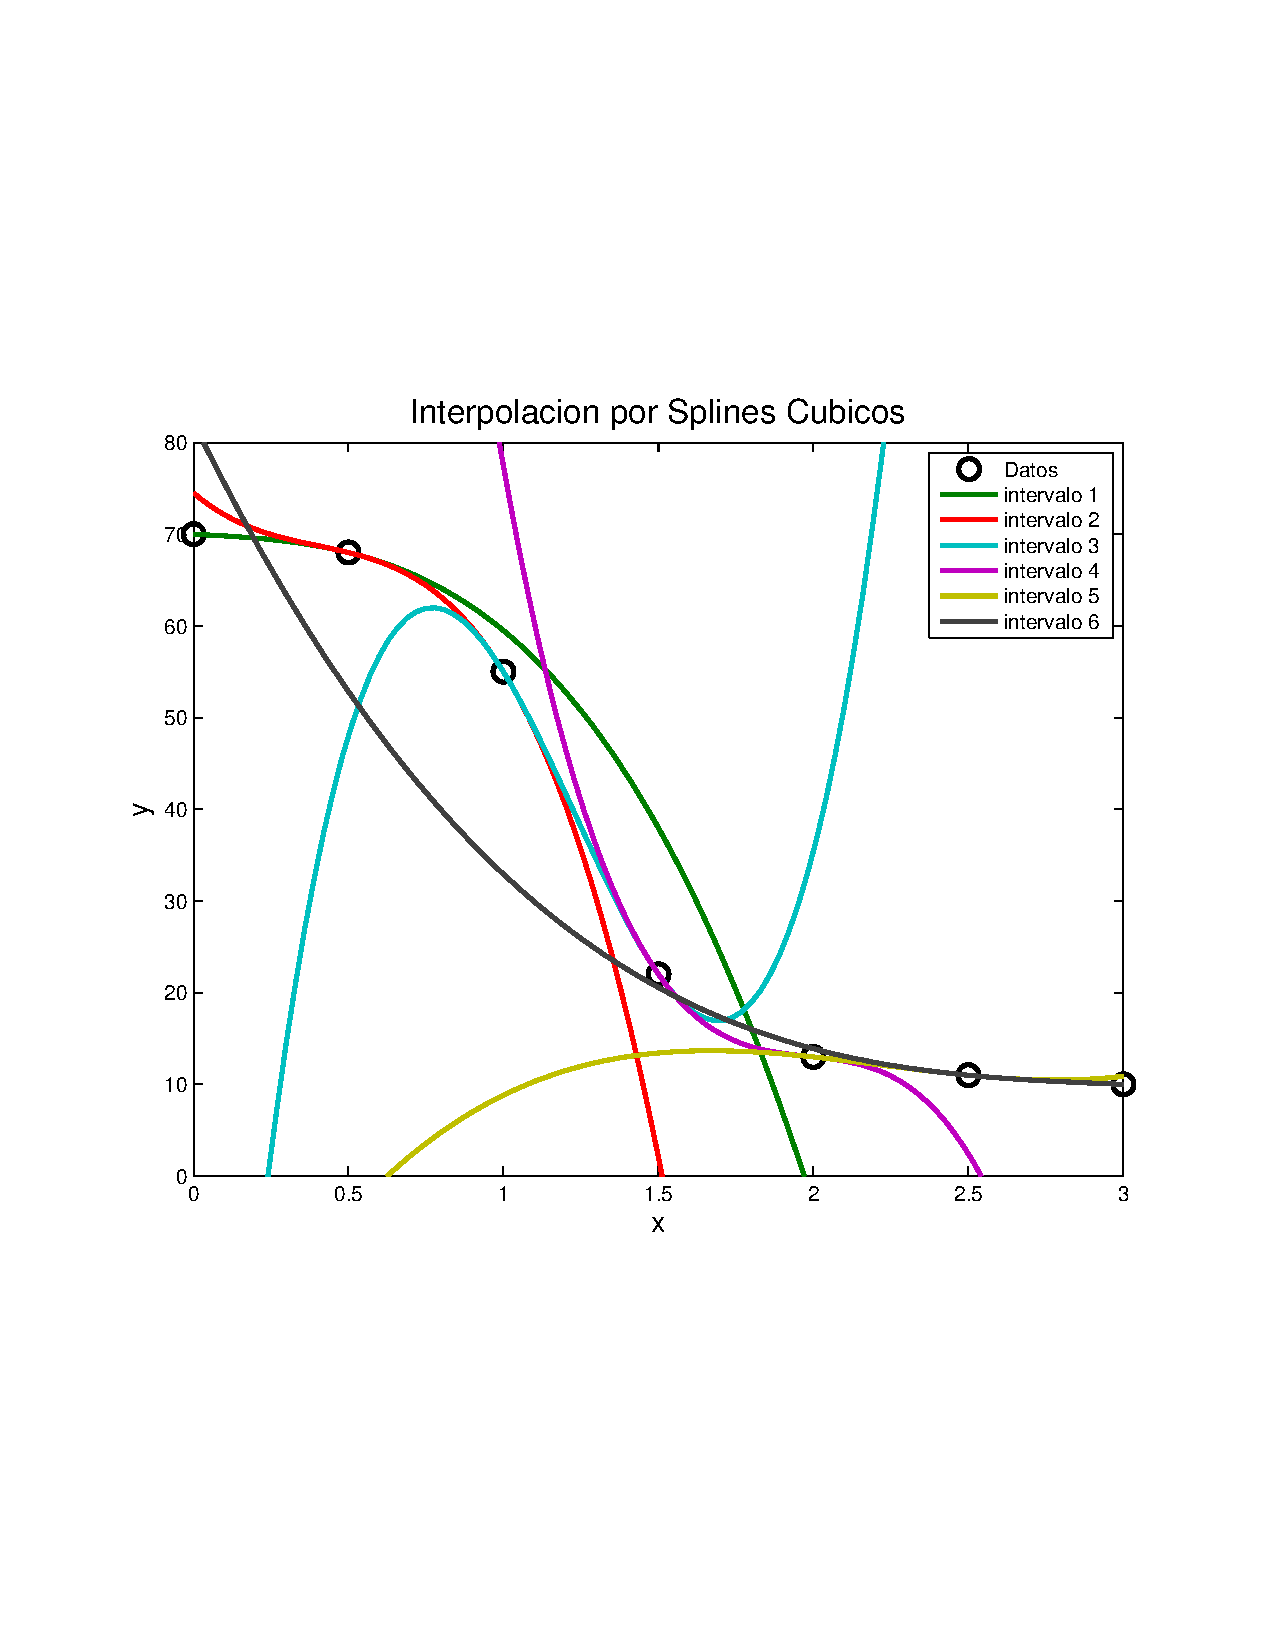
\includegraphics[width=0.6\textwidth,trim=1cm 7cm 1cm 6cm]{./scplines.pdf}
    \caption{\label{FiguraSplinesExtendidos} Cada polinomio vale solo en su intervalo}
  \end{figure}
\end{frame}

\mode<article>
El problema no ha terminado aún. El Enunciado pide, en pocas palabras,
encontrar la profundidad a la que se minimiza la derivada primera
de la función, que será cuando la derivada segunda se anule.
Hay varias maneras de resolver esto. 

En primera instancia, uno podría pensar que la derivada estara bien
representada por la derivada de los polinomios. Esta hipótesis se 
maneja en la \autoref{FiguraDerivPoli}. El problema es que los
polinomios son a lo sumo dos veces derivables, pero lasegunda derivada
si bien es continua es ``aserrada'' de manera que la aproximación
a su cero puede ser tan buena o mala como nuestra tolerancia a
los errores.

\begin{figure}
  \includeslide[width=\textwidth]{FrameFigDerivPoli}
  \caption{\protect\label{FiguraDerivPoli}}
\end{figure}

\mode*
\begin{frame}<presentation>[label=FrameFigDerivPoli]
  \frametitle{Derivar polinomios}
  \center
  \includegraphics[width=0.8\textwidth,page=6,trim=0cm 0cm 0cm 4.1cm,clip]{./Resumen/GUIA1-Resumen-2018.pdf}

\end{frame}

\mode<article>
Otra forma de resolver el problema seria derivar numéricamente los datos
como  se muestra en la \autoref{FigureDerivarDatos}. Notar que con 
este truco se obtienen derivadas suaves, pero las derivadas 
numéricas tienen su error intrínseco y nuevamente es nuestra
tolerancia a los errores la que determinará la confianza que le 
tengamos al resultado. 

no lo hemos dicho, pero el lugar donde se anula la derivada 
segunda podemos encontrarlo usando algún algoritmo 
de optimización. Por ejemplo el método de bisección. 

\begin{figure}
  \includeslide[width=\textwidth]{FrameFigureDerivarDatos}
  \caption{\protect\label{FigureDerivarDatos} Solucion del problema al
  derivar numéricamente los datos}
\end{figure}

\mode*
\begin{frame}<presentation>[label=FrameFigureDerivarDatos]
  \frametitle{Interpolar la derivada numérica de los datos}
  \center
  \includegraphics[width=0.8\textwidth,page=7,trim=0cm 0cm 0cm 4.2cm,clip]{./Resumen/GUIA1-Resumen-2018.pdf}
\end{frame}

\mode*
 
\mode<all>

